\chapter{Transporte de portadores de carga}

Los electrones y huecos en movimiento pueden producir una corriente eléctrica. La corriente I es el movimiento de carga Q en función del tiempo t: un amperio equivale a un coulomb por segundo. Esto se puede describir por medio de la siguiente ecuación:

\[ I = \dfrac{Q}{t} \]

En los semiconductores existen dos mecanismos de transporte de portadores de carga. El primero es el \textbf{arrastre}, debido a la aplicación de un campo eléctrico. El segundo es la \textbf{difusión}, debido a gradientes de concentración de portadores de carga. En este capítulo se estudian ambos fenómenos.

\section{Arrastre}

En un semiconductor sin campo eléctrico aplicado, los electrones se mueven de manera aleatoria sin dirección definida (movimiento browniano). El flujo neto es cero.

\[ I = 0 \]

Una partícula cargada experimenta una fuerza al ser sometida a un campo eléctrico externo.

\[ \vec{F} = m \cdot \vec{a} \]

Un electrón aislado, en presencia de campo eléctrico, experimenta una aceleración constante, por lo que la velocidad incrementa:

\[ \vec{F} = -q \cdot \vec{E} = m \cdot \dfrac{d\vec{v}}{dt} \]

Dentro de un material, la velocidad que se produce no es la misma, debido a colisiones de electrones con la red cristalina y a fuerzas de atracción y repulsión. La velocidad resultante en un cristal es constante y se conoce como \textbf{velocidad de arrastre}:

\[ \vec{v}_d = \mu \cdot \vec{E} \]

La constante $\mu$ es la \textbf{movilidad} de los portadores dentro del cristal, y tiene un valor aproximado de $\mu_n = 1350\ cm^2/Vs$ para electrones, o de $\mu_p = 480\ cm^2/Vs$. Estos valores dependen de la tecnología.

Los electrones tienen una movilidad mayor que los huecos, siendo mayor por un factor de alrededor de 3. Esto quiere decir que, para un mismo campo eléctrico, los electrones son 3 veces más rápidos que los huecos.

La movilidad está determinada por la masa efectiva, la dispersión por impurezas y la dispersión por la estructura cristalina.

\subsection{Corriente de arrastre}

La \textbf{corriente de arrastre} (\textit{drift}) es la que se produce cuando se aplica una tensión externa, y está relacionada con la Ley de Ohm. En circuitos eléctricos simples, la \textbf{corriente convencional} es la que sale de la terminal positiva de la fuente, y retorna por la terminal negativa. Sin embargo, la \textbf{corriente de electrones} tiene dirección opuesta a la corriente convencional: los electrones salen de la terminal negativa y fluyen hacia la terminal positiva de la fuente.

Para derivar la ecuación de corriente de arrastre, considere el diagrama de la Figura 11. Si se aplica una tensión V a una barra con dimensiones $w$, $l$, $h$, y la tensión se aplica en la dirección longitudinal, la corriente de arrastre se calcula como la cantidad de electrones que atraviesan un plano con área transversal $A=w\times{}h$ en un determinado instante de tiempo $\Delta{}t$.

\begin{figure}[H]
    \centering
    \includegraphics{figuras/corriente_arrastre.png}
    \caption{Corriente de arrastre: corriente convencional y corriente de electrones.}
    \label{corriente_arrastre}
\end{figure}

La corriente que fluye por la barra es:

\[ I = \dfrac{Q}{\Delta{}t} \]

La carga total que está encerrada en el volumen marcado es $Q=q \cdot n \cdot w \cdot h \cdot \Delta \vec{l}$:

\[ I = \dfrac{q \cdot n \cdot w \cdot h \cdot \Delta \vec{l}}{\Delta{}t} \]

Los electrones se mueven a una velocidad $\vec{v} = d\vec{l}/dt = \Delta{}l/\Delta{}t$:

\[ I = q \cdot n \cdot w \cdot h \cdot \vec{v} \]

La velocidad de arrastre es $\vec{v} = \mu_n \cdot \vec{E}$:

\[ I = q \cdot n \cdot w \cdot h \cdot \mu_n \cdot \vec{E} \]

El área transversal de la barra es $\vec{A} = w \cot h$:

\[ I = q \cdot n \cdot \vec{A} \cdot \mu_n \cdot \vec{E} \]

La densidad de corriente se define como $J=I/A$:

\[ J_n = q \cdot n \cdot \mu_n \cdot \vec{E} \]

Además, se debe considerar la contribución de los huecos a la corriente de arrastre. Los huecos se mueven en dirección opuesta, pero su carga también es opuesta, por lo que la densidad de corriente total tiene la misma dirección que la corriente convencional, y se calcula como:

\[ \vec{J}_{drift} = \vec{J}_n + \vec{J}_p = q n \mu_n \vec{E} + q p \mu_p \vec{E} \]

La corriente de arrastre en un material se calcula como:

\[ \vec{J}_{drift} =  \sigma \vec{E} \]

Por lo que la conductividad de un material se puede calcular como:

\[ \sigma = q n \mu_n + q p \mu p \]

La resistividad es el inverso de la conductividad:

\[ \rho = \dfrac{1}{q n \mu_n + q p \mu p} \]

En materiales de tipo n se cumple que $n \gg p$, de modo que:

\[ \rho \approx \dfrac{1}{q n \mu_n} \]

Mientras que, en materiales de tipo p, se cumple que $p \gg n$, de modo que:

\[ \rho \approx \dfrac{1}{q p \mu_p} \]

Esto indica que en materiales de tipo n, la mayoría de la corriente se obtiene gracias al movimiento de electrones, que se denominan los \textbf{portadores mayoritarios} en este material, por estar en mayor cantidad. Los huecos en un material de tipo n son los \textbf{portadores minoritarios} y su contribución a la corriente total es despreciable.

En un material de tipo p, los huecos son los \textbf{portadores mayoritarios}, la totalidad de la corriente es producida por los huecos, los electrones son los \textbf{portadores minoritarios}, y la contribución de los electrones a la corriente de arrastre total es despreciable.

\begin{ejemplo}
Una barra de silicio está dopada uniformemente con arsénico, con una concentración de dopado $N_D=10^{12}\ cm^{-3}$. La barra tiene dimensiones $l=1\ cm$, $w=5\ mm$ y $h=1\ mm$. Se aplica una tensión $V=1\ V$ en dirección longitudinal. Determine la concentración de electrones y huecos, la resistividad, la conductividad, la densidad de corriente de arrastre y la corriente total que fluye por la barra.
\end{ejemplo}

\begin{solucion}
Las concentraciones de electrones y huecos son:

\[ n \approx N_D = 10^{12}\ cm^{-3} \]

\[ p \approx \dfrac{{n_i}^2}{n} = \dfrac{(10^{10})^2}{10^{12}} = 10^8\ cm^{-3} \]

La conductividad de la barra se calcula como:

\[ \sigma = q n \mu_n + q p \mu_p \]

\[ \sigma = q (n \mu_n + p \mu_p) \]

\[ \sigma = (1.602\times{}10^{-19}\ C) (10^{12}\ cm^{-3} \cdot 1350\ cm^2/Vs + 10^8\ cm^{-3} \cdot 480\ cm^2/Vs) \]

\[ \sigma = 2.613\times{}10^{4}\ \dfrac{C}{cm\cdot{}V\cdot{}s} \]

\[ \sigma = 2.613\times{}10^{4}\ S/cm \]

La resistividad es el inverso de la conductividad:

\[ \rho = \dfrac{1}{\sigma} = 4623.8\ \Omega \cdot cm \]

El campo eléctrico aplicado es:

\[ \vec{E} = \dfrac{V}{\vec{l}} = \dfrac{1\ V}{1\ cm} = 1\ V/cm \]

La densidad de corriente de arrastre es:

\[ \vec{J} = \sigma \cdot \vec{E} = (2.613\times{}10^4\ S/cm) \cdot (1\ V/cm) \]

\[ \vec{J} = 2.613\times{}10^{-4}\ A/cm^2 \]

La corriente total se obtiene como:

\[ I = \vec{J} \times{} \vec{A} = (2.613 \times 10^{-4}\ A/cm^2) \cdot{} (0.1\ cm \times 0.5\ cm) \]

\[ I = 10.815\ \mu A \]
\end{solucion}


\subsection{Saturación de velocidad de arrastre}

En ausencia de campo eléctrico, el electrón presenta un movimiento térmico aleatorio con una velocidad térmica promedio $v_t$. Al aplicar un campo eléctrico externo, el electrón adquiere una velocidad de arrastre determinada por:

\[ \vec{v}_d = \mu \cdot \vec{E} \]

Esto se cumple para campos eléctricos bajos, con una magnitud inferior a 5 kV/cm aproximadamente. Si se aplica un campo eléctrico más alto, la velocidad de arrastre se satura a un valor de $v_{d,sat} = 10^7\ cm/s$.

La velocidad de arrastre no puede aumentar de manera indefinida debido a las colisiones entre los electrones contra los átomos de la red cristalina, y a las fuerzas de atracción y repulsión entre electrones y dopantes ionizados. Además existen fuerzas entre electrón-electrón que no son consideradas en este análisis.

El efecto de saturación se modela por medio de la siguiente ecuación:

\[ \vec{v}_d = \dfrac{\mu_0}{1+ \dfrac{\mu_0 {E}}{{v}_{d,sat}} } \times \vec{E} \]

Donde la movilidad efectiva es:

\[ \mu = \dfrac{\mu_0}{1+ \dfrac{\mu_0 {E}}{{v}_{d,sat}} } \]

Como se observa, la movilidad depende del campo eléctrico.


\begin{ejemplo}
Un trozo de silicio tiene una longitud de 0.2 $\mu$m y se aplica una tensión de 1 V. Considere $\mu_n = 1350\ cm^2/Vs$ y $v_{d,sat}=10^7\ cm/s$. Determine la movilidad efectiva bajo estas condiciones.
\end{ejemplo}

\begin{solucion}
\[ \vec{E} = \dfrac{V}{\vec{l}} = \dfrac{1\ V}{0.2\ \mu m} \times \dfrac{10^{4}\ \mu m}{1\ cm} = 50000\ V/cm \]

\[ \mu = \dfrac{\mu_0}{1+ \dfrac{\mu_0 {E}}{{v}_{d,sat}} } = \dfrac{1350\ cm^2/Vs}{1+ \dfrac{1350\ cm^2/Vs \cdot {50000\ V/cm}}{10^7\ cm/s} } = 174.19\ cm^2/Vs \]

Los resultados obtenidos en este problema muestran que los dispositivos modernos operan con saturación de velocidad, debido a que las dimensiones son menores a 10 nm.
\end{solucion}


%\subsection{Movilidad en función del dopado}

%La movilidad de electrones ($\mu_{n}$) y huecos ($\mu_{p}$) no es constante; varía de acuerdo al dopaje del semiconductor. El dopado modifica la movilidad de los portadores, de acuerdo con la siguiente ecuación:

%\[ \mu =  \mu_{min} + \dfrac{\mu_0}{1+\left( \dfrac{N}{N_{ref}} \right)^\alpha } \]

%Donde $N$ es la concentración total de dopantes $N_D+N_A$, $N_{ref}$ la concentración de referencia de portadores, $\mu_{o}$ movilidad al vacío y $\mu_{min}$ movilidad mínima. En el caso de dopado con donadores lo valores son: $\alpha=0.91$, $\mu_{min}=92$ cm$^{2}$/$Vs$, $N_{ref}=1.3x10^{17}$ cm$^{-3}$ y $\mu_{o}=1268$ cm$^{2}$/$Vs$. Por otro lado en el dopado con aceptores los valores son: $\alpha=0.88$, $\mu_{min}=54.3$ cm$^{2}$/$Vs$, $N_{ref}=2.35x10^{17}$ cm$^{-3}$ y $\mu_{o}=406.9$ cm$^{2}$/$Vs$

%Ejemplo: movilidad en función del dopado.

%Considerando los valores de referencia disponibles en la siguiente tabla, escriba un script en MATLAB que permita graficar la movilidad tanto de electrones como de huecos, en función de la concentración de dopado, para dopados entre $10^{13}$ y $10^{19}$ cm$^{-3}$.


%\subsection{Movilidad en función de la temperatura}

%La temperatura también modifica la movilidad, como se observa en las siguientes gráficas.


\newpage
\section{Difusión}

La \textbf{difusión} es el movimiento de partículas debido a gradientes de concentración. La Ley de Fick establece que una partícula (no necesariamente cargada) experimenta una fuerza proporcional al gradiente de concentración $\nabla \eta$, y a una constante de proporcionalidad conocida como el \textbf{coeficiente de difusión} $D$:

\[ F = -D \cdot \nabla \eta \]

Donde: 

\begin{itemize}
    \item D: coeficiente de difusión (cm$^2$/Vs)
    \item $\eta$: concentración de las partículas que se difunden (cm$^{-3}$)
    \item $\nabla \eta$: gradiente de concentración
\end{itemize}

La difusión es un fenómeno que ocurre en muchos sistemas físicos, el ejemplo clásico es el de una botella de perfume que se deja destapada en la esquina de una habitación sin ventilación. Después de mucho tiempo, la concentración del perfume en el aire es la misma en toda la sala. Otro ejemplo es el de una gota de tinta en un recipiente con agua: sin necesidad de agitar el agua, la tinta llega a todas partes y se logra una concentración uniforme. Lo mismo ocurre con una bolsa de té en agua caliente. Conforme pasa el tiempo, la sustancia que está más concentrada se difunde, aunque el medio esté completamente quieto.

Esto mismo sucede con los electrones y los huecos: se mueven por difusión de acuerdo con los gradientes de concentración. El efecto no es explicado por repulsión o atracción electrostática, sino que el simple movimiento térmico aleatorio, también conocido como \textbf{movimiento browniano}, reparte las partículas hasta que la concentración llega a ser uniforme en todo el sólido.

\subsection{El concepto de gradiente}

El \textbf{gradiente} es un operador lineal definido como:

\[ \nabla \eta = \dfrac{\partial \eta}{\partial x} \hat{x} + \dfrac{\partial \eta}{\partial y} \hat{y} + \dfrac{\partial \eta}{\partial z} \hat{z} \]

El gradiente apunta en dirección de menor a mayor concentración, por lo que la Ley de Fick incluye un signo negativo, para indicar que las partículas experimentan una fuerza en dirección de mayor a menor concentración.

\begin{ejemplo}
Indique las unidades que tiene el gradiente de concentración $\nabla n$, de manera que las ecuaciones anteriores sean consistentes, tomando en cuenta que la densidad de corriente se expresa en $A/cm^{2}$ y que el coeficiente de difusión tiene unidades de $cm^2/s$.
\end{ejemplo}





\subsection{Desplazamiento de portadores en difusión}

En un trozo de silicio con concentración homogénea, se establece un punto de referencia $x_{r}$; dado que el movimiento térmico es aleatorio, los portadores no tienen preferencia de dirección, por lo que migra la mitad de ellos hacia la izquierda de $x_{r}$ y la otra mitad hacia la derecha de $x_{r}$, donde $x_{r}$ es la posición de referencia. Tomando en cuenta que el movimiento hacia la izquierda es negativo y hacia la derecha es positivo dado en la Figura \ref{difusion_portadores} \cite{b11}, el flujo de portadores es:

\[ F = \dfrac{P_{i}}{2} - \dfrac{P_{d}}{2} \]

Donde $P_{i}$ es el perfil de portadores del lado izquierdo de $x_{r}$ y $P_{d}$ es el perfil de portadores del lado derecho de $x_{r}$.

\begin{figure}[H]
    \centering
    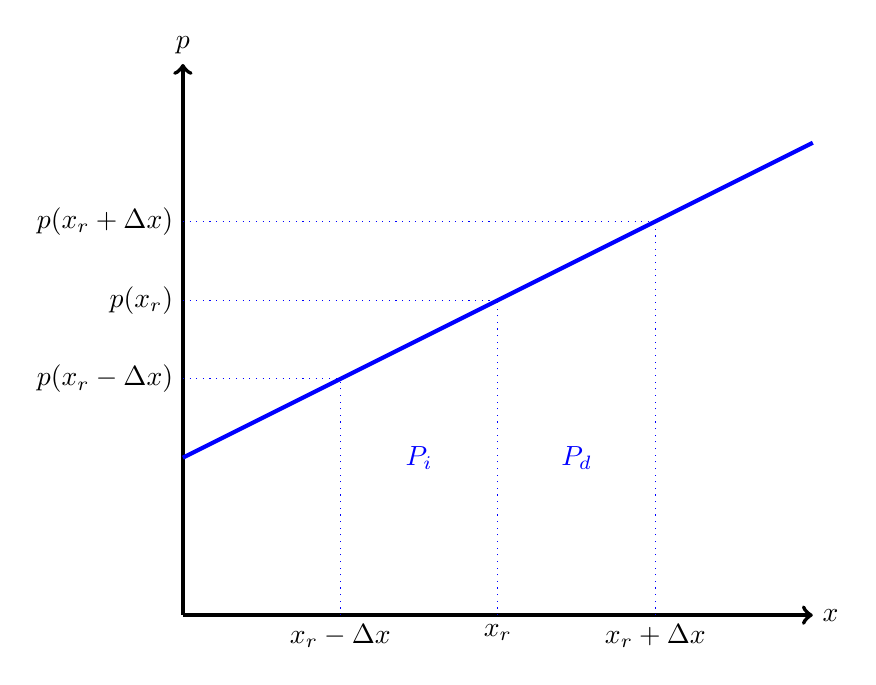
\begin{tikzpicture}
    % Eje X
    \draw[line width=1.5pt,-to]         (0,-2) -- (8,-2);
    \draw (8,-2) node[right] {$x$};
    % Eje Y
    \draw[line width=1.5pt,-to]         (0,-2) -- (0,5);
    \draw (0,5) node[above] {$p$};
    % Ecuacion de p(x)
    \draw[color=blue, line width=1.5pt] (0,0)  -- (8,4);
    % Lineas a eje x
    \draw[color=blue,dotted]            (2,-2) -- (2,1);
    \draw[color=blue,dotted]            (4,-2) -- (4,2);
    \draw[color=blue,dotted]            (6,-2) -- (6,3);
    % Lineas a eje y
    \draw[color=blue,dotted]            (0,1) -- (2,1);
    \draw[color=blue,dotted]            (0,2) -- (4,2);
    \draw[color=blue,dotted]            (0,3) -- (6,3);
    % Valores en eje x
    \draw (2,-2) node[below] {$x_r - \Delta x$};
    \draw (4,-2) node[below] {$x_r$};
    \draw (6,-2) node[below] {$x_r + \Delta x$};
    % Valores en eje y
    \draw (0,1) node[left] {$p(x_r - \Delta x)$};
    \draw (0,2) node[left] {$p(x_r)$};
    \draw (0,3) node[left] {$p(x_r + \Delta x)$};
    % Anotaciones en el grafico
    \draw[color=blue] (3,0) node[] {$P_i$};
    \draw[color=blue] (5,0) node[] {$P_d$};
    \end{tikzpicture}
    \caption{Difusión de portadores con gradiente de concentración.}
    \label{difusion_portadores}
\end{figure}

Ante diferencias de concentración en un trozo de silicio y considerando que las concentraciones se difunden del punto de mayor concentración al de menos; se obtendrá un flujo neto negativo al tener mayor concentración del lado derecho de $x_{r}$.

Los cambios de concentración no son necesariamente lineales pero si se toma un $\Delta x$ muy pequeño, como el promedio de recorrido de un portador $\lambda$ se puede linealizar mediante series de expansión de Tayor:

\[ n(x_{r}+\Delta x) = n(x_{r}) + \dfrac{dn}{dx}|_{x=x_{r}} \Delta x \]

Si se analiza el lado izquierdo de $x_{r}$ de la pieza, se tiene:

\[ P_{i} = A\lambda \dfrac{n(x_{r}-\Delta x) - n(x_{r})} {2} \]

Considerando la seria de expansión de Taylor y un $\Delta x= \lambda$, de forma tal que el portador pueda atravesar la región:

\[ P_{i} = \dfrac{A\lambda}{2} \left[ n(X_{r}) - \dfrac{dn}{dx} |_{x=x_{r}} \lambda + n(x_{r}) \right] = \dfrac{A\lambda}{2} \left[ 2 n(x_{r}) - \dfrac{dn}{dx} |_{x=x_{r}} \lambda \right]\]

De forma similar el lado derecho de $x_{r}$, se puede escribir:

\[ P_{d} = \dfrac{A\lambda}{2} \left[ 2 n(x_{r}) + \dfrac{dn}{dx} |_{x=x_{r}} \lambda \right]\]

Mediante la descripción de flujo se puede extraer la densidad de corriente por unidad de tiempo y de área transversal en una sola dimensión:

\[ J_{dif,n} = \dfrac{q}{A \tau} \left[ \dfrac{P_{i}}{2} - \dfrac{P_{d}}{2} \right] = -q D_{n} \dfrac{dn}{dx} |_{x=x_{r}} \]

Con: 

\[ D_{n} = \dfrac{\lambda^{2}}{2 \tau}  \]

\subsection{Corriente de difusión}

Para semiconductores de tipo $p$ se tiene:

\[ \vec{J}_{dif,p} = -q \cdot D_p \cdot \nabla p \]

Observe el signo que tiene la ecuación, el cual es el mismo que aparece en la ley de Fick. Esto significa que la corriente de huecos (corriente convencional de cargas positivas) tiene dirección opuesta al gradiente de concentración de huecos. 

Considere ahora el caso de semiconductores de tipo $n$:

\[ \vec{J}_{dif,n} = +q \cdot D_n \cdot \nabla n \]

Si la concentración de portadores varía sólo en una dimensión:

\[ \vec{J}_{dif,p} = - q D_p \dfrac{dp}{dx} \hat{x} \]

\[ \vec{J}_{dif,n} = q D_n \dfrac{dn}{dx} \hat{x} \]

Donde se debe resaltar el signo positivo que tiene la ecuación, contrario al que indica la ley de Fick. Esto sucede porque la corriente de electrones (corriente técnica de cargas negativas) produce una corriente convencional en sentido opuesto, de modo que se debe invertir el signo de la ley de Fick para ser consistentes con la definición de corriente convencional.

La corriente de difusión total en una dimensión se calcula matemáticamente como:

\[ \vec{J}_{dif} = \vec{J}_{dif,n} + \vec{J}_{dif,p} \]

\subsection{Relación de Einstein}

La movilidad está relacionada con el coeficiente de difusión por medio de la relación de Einstein:

\[ D = V_t \cdot \mu \]

Los coeficientes de difusión de electrones y huecos tienen valores conocidos. Para el silicio se tiene que $D_n=34.90\ cm^2/s$ mientras que $D_p=12.41\ cm^2/s$. Las unidades son arbitrarias ya que estas son constantes de proporcionalidad, determinadas experimentalmente.

\begin{ejemplo}
Verifique el valor de los coeficientes de difusión $D_n$ y $D_p$, conociendo que para silicio $\mu_n = 1350\ cm^2/Vs$, $\mu_p = 480\ cm^2/Vs$ y que el voltaje térmico a temperatura ambiente es $V_t = 25.85\ mV$.
\end{ejemplo}

\begin{solucion}
\[ D_n = (25.85\ mV) \cdot (1350\ cm^2/Vs) = 34.90\ cm^2/s \]

\[ D_p = (25.85\ mV) \cdot (480\ cm^2/Vs) = 12.41\ cm^2/s \]
\end{solucion}


% \begin{ejemplo}
% Una barra de silicio está dopada uniformemente con boro, con una concentración de dopado $N_A = 10^{16}\ cm^{-3}$. La barra tiene una longitud l=1 cm y un área transversal $A=0.05\ cm^2$. La concentración de huecos es uniforme en toda la barra. 
% 
% Se inyectan electrones de manera constante en el extremo izquierdo, con una concentración de 1000 veces la concentración original de electrones $n_0=(n_i^2)/p=10^4\ cm^{-3}$, con lo que se obtiene el siguiente perfil de concentración:
% 
% \begin{figure}[H]
%     \centering
%     \includegraphics{figuras/ejemplo_corriente_difusion.png}
%     \caption{Perfil de concentración de electrones.}
%     \label{ejemplo_difusion}
% \end{figure}
% 
% Calcule la densidad de corriente de difusión y la corriente total.
% \end{ejemplo}
% 
% \begin{solucion}
% La densidad de corriente de difusión es:
% 
% \[ \vec{J} = -q D_n \nabla n \]
% 
% \[ \vec{J} = -q D_n \dfrac{dn}{dx} \hat{x} \] 
% 
% \[ \vec{J} = -q D_n \dfrac{(n_2-n_1)}{(x_2-x_1)} \hat{x} \] 
% 
% \[ \vec{J} = -(-1.602 \times 10^{-19}\ C)(34.9\ cm^2/s)((10^4-10^7\ cm^{-3})/(1\ cm-0)) \hat{x} \] 
% 
% \[ \vec{J} = -(-1.602 \times 10^{-19}\ C)(34.9\ cm^2/s)(-9.99 \times{} 10^6\ cm^{-4}) \hat{x} \] 
% 
% \[ \vec{J} =5.585 \times 10^{-11}\ A/cm^2 \]
% 
% La corriente total es:
% 
% \[ I = \vec{J} \times \vec{A} = (5.585 \times 10^{-11}\ A/cm^2) \cdot (0.05\ cm^2) \]
% 
% \[ I = 2.79 \times 10^{-12}\ A = 2.79\ pA \]
% \end{solucion}


\subsection{Sonda de punto caliente}

Este experimento permite determinar si una oblea es de tipo P o de tipo N, al colocar dos puntas de prueba sobre la superficie de la oblea. Una de las puntas está a la misma temperatura de la oblea, mientras que la otra se calienta con el propósito de inducir generación térmica de portadores en el punto de contacto.

Si la oblea es de tipo P, al tocar con la punta caliente se crean huecos, los cuales se difunden alejándose, produciendo una región ligeramente negativa y una corriente técnica que sale de la sonda caliente.

Por el contrario, si la oblea es de tipo N, el contacto de la punta caliente crea electrones, los cuales también se difunden alejándose, produciendo una región ligeramente positiva y una corriente técnica en sentido contrario, es decir, entrando por la sonda caliente.

El galvanómetro permite detectar estas corrientes con direcciones opuestas.


%\newpage
%\section*{Problemas}

%\textbf{Problema 3.1.} Una barra de silicio tiene dimensiones de $10 \times 5 \times 4$ $\mu$m. La barra está dopada de manera uniforme, con una concentración de huecos de $10^{15}\ cm^{-3}$. Se aplica una tensión de 1 V entre las terminales de la barra, según se muestra en la figura adjunta. Para estas condiciones, calcule:

%\begin{itemize}
%    \item La concentración de portadores de carga minoritarios.
%    \item La densidad de corriente $J_{drift}$.
%    \item La corriente total en la barra $I$.
%    \item La velocidad de arrastre $v_d$ de electrones.
%    \item La velocidad de arrastre $v_d$ de huecos.
%\end{itemize}


%\textbf{Problema 3.2.} Se inyectan huecos de manera constante en una región de silicio de tipo n. En estado estable, se establece el perfil de concentración de huecos mostrado en la figura adjunta. Encuentre:

%\begin{itemize}
%    \item La magnitud, dirección y unidades del gradiente de concentración $\nabla p$.
%    \item La densidad de corriente de difusión $J_{diff}$.
%\end{itemize}


